\section{Artificial Neural Networks}
Artificial neural networks are a computing system inspired by biological neurons. Neural networks are comprised of neurons which are capable of taking any number of numerical inputs and outputs a numerical value.

\tikzset{%
	every neuron/.style={
		circle,
		draw,
		minimum size=1cm
	},
	neuron missing/.style={
		draw=none, 
		scale=4,
		text height=0.333cm,
		execute at begin node=\color{black}$\vdots$
	},
}

\begin{figure}[t]
	\centering
	\resizebox{0.6\textwidth}{!}{
		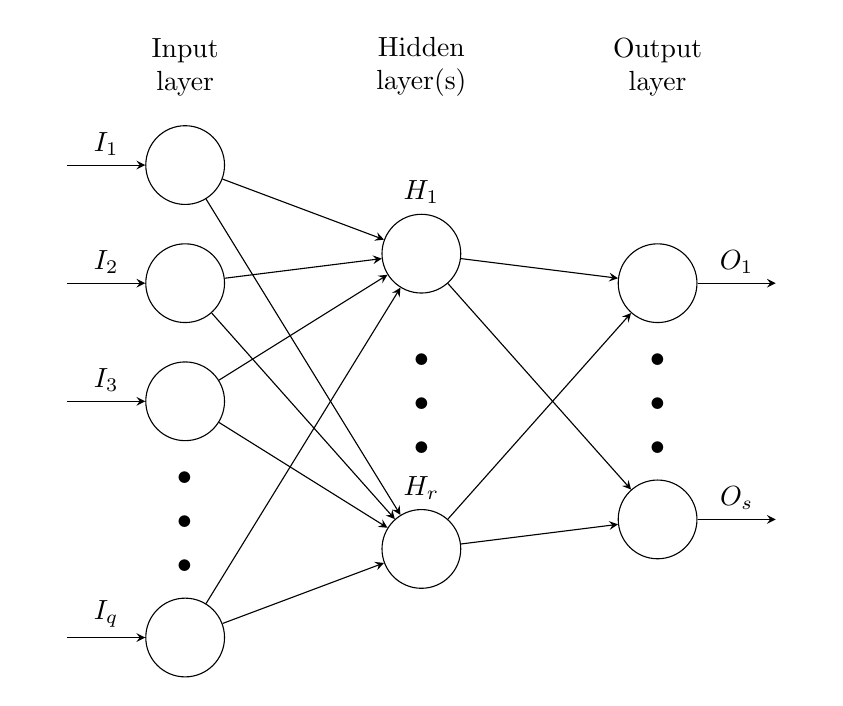
\begin{tikzpicture}[x=1.5cm, y=1.5cm, >=stealth]
			% Input neurons
			\foreach \m/\l [count=\y] in {1,2,3,missing,4}
			  \node [every neuron/.try, neuron \m/.try] (input-\m) at (0,2.5-\y) {};
			% Hidden neurons
			\foreach \m [count=\y] in {1,missing,2}
			  \node [every neuron/.try, neuron \m/.try ] (hidden-\m) at (2,2-\y*1.25) {};
			% Output neurons
			\foreach \m [count=\y] in {1,missing,2}
			  \node [every neuron/.try, neuron \m/.try ] (output-\m) at (4,1.5-\y) {};
			% Input labels
			\foreach \l [count=\i] in {1,2,3,q}
			  \draw [<-] (input-\i) -- ++(-1,0)
			    node [above, midway] {$I_\l$};
			% Hidden neuron labels
			\foreach \l [count=\i] in {1,r}
			  \node [above] at (hidden-\i.north) {$H_\l$};
			% Out arrows with labels
			\foreach \l [count=\i] in {1,s}
			  \draw [->] (output-\i) -- ++(1,0)
			    node [above, midway] {$O_\l$};
			% Input to hidden arrows
			\foreach \i in {1,...,4}
			  \foreach \j in {1,...,2}
			    \draw [->] (input-\i) -- (hidden-\j);
			% Hidden to output arrows
			\foreach \i in {1,...,2}
			  \foreach \j in {1,...,2}
			    \draw [->] (hidden-\i) -- (output-\j);
			% Layer labels
			\node [align=center, above] at (0,2) {Input \\ layer};
			\node [align=center, above] at (2,2) {Hidden \\ layer(s)};
			\node [align=center, above] at (4,2) {Output \\ layer};
		\end{tikzpicture}
	}
	\caption[Artificial Neural Networks]{A Visualization of how neurons interact within an artificial neural network. In this example, the network has 3 layers: An input layer, a hidden layer, and an output layer. The input layer consists of $q$ neurons, each having one input value. Each of these inputs neurons are connected to each of the $r$ neuron in the hidden layer. Each neuron in the hidden layer is also connected to each neuron in the output layer. Finally, the output layer contains $s$ neurons and returns $s$ output values.}\label{fig:background-neuralnet}
\end{figure}

Mathematically, a single neuron is a function.
The function of a neuron $j$ receiving input $x_j$ and producing output $y_j$ is composed of the activation $a_j$, an activation function $f_a$ which returns the activation, and an output function $f_{o}$.
The activation $a_j$ can also be considered the neuron's state.
The activation function $f_a$ calculates $a_j$ given the network input $x_j$ and can be defined as:
\begin{align}
	a_j &= f_a\left(x_j\right)
\end{align}
The output function $f_o$ computes $y_j$ based on $a_j$ and is defined as:
\begin{align}
	y_j &= f_o\left(a_j\right)
\end{align}
Many activation functions exists and are used including the identity function and the rectified linear unit (ReLU), defined as:
\begin{align}
	f_a(x) &= 
	\begin{cases}
		0	& \text{for } x \leq 0\\
		x	& \text{for } x > 0
	\end{cases}
\end{align}

Between each neuron in the network are connections which transfer the output of neuron $i$ to neuron $j$. Each of these connections are assigned a weight $w_{ij}$, which is computed by the learning algorithm.
Each neuron also has a bias $w_{0j}$.
These parameters are used to provide a neuron its input $x_j$. This is defined as:
\begin{align}
	x_j &= \sum_{i}y_iw_{ij} + w_{0j}
\end{align}

\figref{fig:background-neuralnet} shows a visualization of the interactions between multiple neurons.

Learning occurs by using an algorithm known as backpropagation to modify the parameters of the neural network.
Further discussion on backpropagation can be found in Section \ref{section:background-backpropagation}.

Deep neural networks are so called deep due to having multiple "hidden" layers between the input and output which are not accessed directly.

\subsection{Convolutional Neural Networks}\label{section:background-cnn}
Convolutional Neural Networks (CNNs) are a specific class of deep neural networks and have been found to perform exceptionally well for image analysis, such as image classification and segmentation.
The inspiration for CNNs come from biological processes to simulate the organization of the visual cortex in animals~\cite{cnnbiology}.
Convolutional layers are the core building blocks of CNNs.
These convolutional layers consist of a set of learnable filters which are convolved across the entire input and compute the dot products between the different entries of the filter.

\definecolor{cred}{RGB}{155,47,47}
\definecolor{cblue}{RGB}{40,79,168}
\definecolor{cgreen}{RGB}{78,131,65}

% Elements of matrix 1
\def\elementsa{{2, 3, 3, 2, 2,
				7, 8, 5, 9, 0,
				2, 4, 7, 5, 4,
				4, 4, 0, 0, 6,
				9, 6, 5, 9, 3}}
% Elements of the convolution
\def\elementsb{{0, 1, 0, 
				1, 0, 1, 
				0, 1, 0}}

\def\elementsc{{19, 27, 12,
				21, 14, 20,
				14, 16, 20}}
\begin{figure}[t]
	\centering
	\resizebox{0.7\textwidth}{!}{
		\begin{tikzpicture}
			[x={(0.866cm,0.5cm)}, y={(-0.866cm,0.5cm)}, z={(0cm,1cm)}, scale=0.8]			
			% Matrix A
			\begin{scope}[canvas is xz plane at y=0,transform shape]
				
				\foreach \ii [count = \xi] in {1,2,3,4,5}{
		    		\foreach \jj  [count = \yi]in {1,2,3,4,5}{
		    			\pgfmathsetmacro{\nn}{int(\xi+5*\yi-5)}
						\node[cred,draw,minimum size=1cm] (n\nn-1) at (\ii,-\jj) {
							\pgfmathparse{\elementsa[(5*(\yi-1))+(\xi-1)]}\pgfmathresult
						};
					}
				}
				\node[cred,draw,minimum size=1cm,above=of n1-1.west,anchor=west] {matrix $A$};  % Matrix Label
			\end{scope}
			
			% Matrix B
			\begin{scope}[canvas is xz plane at y=-5.5,transform shape]
				\foreach \ii [count = \xi] in {1,2,3}{
		   			\foreach \jj  [count = \yi]in {1,2,3}{
				     	\pgfmathsetmacro{\nn}{int(\xi+3*\yi-3)}
				     	\pgfmathsetmacro{\val}{}]
						\node[cblue,draw,minimum size=1cm] (n\nn-2) at (\ii,-\jj) {
							\pgfmathparse{\elementsb[(3*(\yi-1))+(\xi-1)]}\pgfmathresult
						};
					}
				}
				\node[cblue,draw,minimum size=1cm,above=of n1-2.west,anchor=west] {matrix $B$};  % Matrix Label
			\end{scope} 
			
			% Matrix C
			\begin{scope}[canvas is xz plane at y=-9,transform shape]
				\foreach \ii [count = \xi] in {1,2,3}{
		   			\foreach \jj  [count = \yi]in {1,2,3}{
				    	\pgfmathsetmacro{\nn}{int(\xi+3*\yi-3)}
						\node[cgreen,draw,minimum size=1cm] (n\nn-3) at (\ii,-\jj) {
							\pgfmathparse{\elementsc[(3*(\yi-1))+(\xi-1)]}\pgfmathresult
						};
					}
				}
				\node[cgreen,draw,minimum size=1cm,above=of n1-3.west,anchor=west] {matrix $C$};  % Matrix Label
			\end{scope} 
			
			% Top of box
			\draw[fill=red!50,opacity=0.3] (n3-1.north east) -- (n3-2.north east) --(n1-3.north east)
			--(n1-3.north west)-- (n1-2.north west) --  (n1-1.north west)  ;
			
			% Bottom of box
			\draw[fill=red!50,opacity=0.3] (n13-1.south east) -- (n9-2.south east) --(n1-3.south east)
			--(n1-3.south west)-- (n7-2.south west)-- (n11-1.south west)  ;    

			% Right side of box			
			\draw[fill=red!50,opacity=0.3] (n3-1.north east) -- (n3-2.north east) --(n1-3.north east)
			--(n1-3.south east)-- (n9-2.south east)-- (n13-1.south east)  ;

			% Left side of box			
			\draw[fill=red!50,opacity=0.3] (n1-1.north west) -- (n1-2.north west) --(n1-3.north west)
			--(n1-3.south west)-- (n7-2.south west)-- (n11-1.south west)  ;      
		
		\end{tikzpicture}
	}
	\caption[Convolution operation]{An example of a how a convolution on matrix $A$ and matrix $B$ would result in matrix $C$.}
\end{figure}

By using multiple convolutional layers, higher level features can be extracted, generating a feature map.
The module responsible for extracting the feature map is commonly known as the encoder.

The convolutional layers that make up the CNN are called the feature encoder.
The output of these convolutional layers are then fed into a module with one or more fully convolutional layers to produce a classification of each pixel in a scene.
These convolutional layers work by taking the deep feature maps produced by the encoder and using deconvolutional or upsampling layers to produce a log-likelihood vector for each pixel.
This module is known as the decoder.
The resulting vector produced is a probability of each pixel being a certain class.
Applying an argmax operation on this vector produces a segmentation of the input image.

A bottleneck structure may also be used to increase performance.
A bottleneck structure in a convolutional neural network reduces the number of features by performing a $1 \times 1$ convolution on a tensor before performing a convolution operation.
A final $1 \times 1$ convolution is then performed to expand the tensor to contain a meaningful combination features.
As the input features are correlated, redundancy can be removed by performing the first $1 \times 1$ convolution.

For example, performing a $3 \times 3$ convolution on a $256 \times 256$ input tensor requires more than 589,000 operations.
A bottleneck structure can be used to reduce the dimensionality of the input tensor to only 64 dimensions using a $1 \times 1$ convolution.
The $3 \times 3$ convolution is then performed on this tensor.
Finally, the resulting tensor is re-expanded back to the original 256 dimensions using another $1 \times 1$ convolution.
This would result in slightly over 69,000 operations, significantly less than without the bottleneck structure.

This reduces both the number of operations required as well as the number of parameters in the network.